\section{Quantum Computing}

Quantum computers use quantum bits (qubits) instead of normal bits that classical computers use.
While a bit can be either in the state $0$ or $1$, a qubit can be in a so-called superposition of two states.
States of qubits are generally written using the Dirac-Notation, also known as the Bra-Ket-Notation
The two states, the superposition is a combination of, are called the basis.
The most basic basis is the basis $\{ \ket{0}, \ket{1} \}$.
The formula (\ref{formula:quantum.superposition}) describes such a superposition.
When one measures the state of the qubit, it collapses into one of the base states, which is the result of the measurement.
The probability of either basis state being measured is the square of the the complex amplitude of the basis state in the superposition.
\cite{Vedral1998}
\begin{subequations}
\begin{align}
  \label{formula:quantum.superposition}
  & \ket{\phi} = \alpha \cdot \ket{0} + \beta \cdot \ket{1}
  & \text{with } \alpha, \beta \in \mathbb{C}, \alpha^2 + \beta^2 = 1
  \\
  & p_0 = \alpha^2
\end{align}
\end{subequations}

Multiple qubits chained together form a quantum register.
In such a register, the measurement results of one qubit might depend on the measurement results of other qubits.
This is called entanglement.
The formula (\ref{formula:quantum.superposition.register}) describes a quantum register with $n$ qubits.
If one can't separate the formula into single qubits, the state is entangled.
The probability of measuring a specific state of the quantum register is given by the amplitude of that state squared.
\cite{Vedral1998}
\begin{subequations}
\begin{align}
  \label{formula:quantum.superposition.register}
  & \ket{\Phi} = \sum_{x \in \{0, 1\}^n} \alpha_x \cdot \ket{x}
  & \text{with } \forall x \in \{0, 1\}^n: \alpha_x \in \mathbb{C},
  \sum_{x \in \{0, 1\}^n} \alpha_x^2 = 1
  \\
  & p_x = \alpha_x^2
\end{align}
\end{subequations}

\subsection{Annealing-based Quantum Computing}
\label{backg:annealing}

Annealing-based quantum computers are designed to tackle optimization problems well.
The quantum processing unit takes an Ising as input and embeds the biases on itself.
For this, it uses couplers between its qubits.
Then quantum tunneling is exploited to find a state of the qubits where the energy of the QPU is minimal.
This is also the state of the Ising model variables that minimize the model.
\cite{Boixo2013}

Ising models and QUBOs are equivalent, and the conversion is computationally inexpensive.
The difference is the domain of the variables.
\cite{Bian2010}
In Ising models, the domain is $\{-1, 1\}$, and in QUBOs, it is $\{0, 1\}$.
This work considers QUBOs rather than Ising models.
The formula \ref{formula:qubo.form} shows the structure of a QUBO.
$a$ are called linear biases because they depend on one variable, and $b$ are called quadratic biases because they depend on two variables.

\begin{align}
  \label{formula:qubo.form}
  E(v) = & \quad
  \sum_i a_i \cdot v_i
  + \sum_{i < j} b_{i, j} \cdot v_i \cdot v_j
  + c
\end{align}

\subsubsection{Hybrid Quantum-annealing}

The number of qubits on a QPU is limited, and so are the couplings between them that the QPU uses to embed quadratic biases.
When a problem has too many variables or quadratic biases, it's impossible to find an embedding for the QPU.
Hybrid Solvers can solve such problems faster than purely classical computers.
\cite{Bernoudy2020}

A Hybrid Solver is an algorithm that runs on a classical computer and a quantum computer.
The classical computer receives the problem and attempts to solve it.
It uses the quantum computer for subproblems that the quantum computer can solve faster.
\cite{Zhang2016}

D-Wave's Advantage system has more than $5, 000$ qubits with $15$-way connectivity.
\cite{D-Wave2020}
It can solve problems with up to $5, 000$ binary variables if the quadratic biases are $\leq 15$ for every variable.
If there are some variables with more quadratic biases, they can be distributed onto different qubits.
At some point, this is not possible anymore, and the Hybrid Solver has to be utilized.
D-Wave's Hybrid Solver can handle fully connected QUBOs of up to $20, 000$ variables.
It can handle non-fully connected QUBOs of up to $1, 000, 000$ variables, but the number of biases has to be smaller than $200, 000, 000$.
\cite{Bernoudy2020}

\subsubsection{Discrete Optimization}

D-Wave also has a Hybrid Solver that can handle problems with discrete variables instead of binary as in QUBOs.
These problems have to be a Discrete Quadratic Model (DQM), which can be written as shown in the formula (\ref{formula:dqm.form}).
The solver can handle a maximum of $5, 000$ variables with up to $10, 000$ cases per variable.
The maximum number of biases is $2, 000, 000, 000$.
\cite{DQMHybrid2020}

\begin{align}
  \label{formula:dqm.form}
  E(v) =
  & \quad \sum_i a_i \cdot v_i + \sum_{i < j} b_{i, j} \cdot \left( v_i \otimes v_j \right) + c
\end{align}

Note that in the formula (\ref{formula:dqm.form}), $a_i$ is a vector that holds the linear biases for the variable $i$.
$a_i \cdot v_i$ is the scalar product of the linear biases with the value of variable $i$.
$b_{i, j}$, on the other hand, is a matrix that holds the quadratic biases of the variable $i$ and $j$.
$b_{i, j} \cdot \left( v_i \otimes v_j \right)$ is the Frobenius Inner Product $\langle b_{i, j}, v_i \otimes v_j \rangle_F$ that is defined as the sum of all elements of both matrices multiplied element-wise.

\subsection{Gate-based Quantum Computing}

In the gate-based model of quantum computers, gates represent the manipulation of qubits.
The qubits and quantum gates form a quantum circuit.

Single qubit gates manipulate only one qubit at a time.
Double qubit gates manipulate two qubits and can entangle two qubits.
The formula (\ref{formula:gate.x}) shows an example of a single qubit gate.
It swaps the amplitudes of the two basis states $\ket{0}$ and $\ket{1}$.
The formula (\ref{formula:gate.cnot}) shows an example of a double qubit gate.
It applies the $X$-gate to the second qubit if the first qubit is in the base state $\ket{1}$.
This entangles both qubits with each other.
\begin{subequations}
\begin{align}
  \label{formula:gate.x}
  X & = \ket{0} \bra{1} + \ket{1} \bra{0}
  & = \begin{pmatrix}
    0 & 1 \\ 1 & 0
  \end{pmatrix}
  \\
  \label{formula:gate.hadamard}
  H & = \frac{1}{\sqrt{2}} \left(
    \left( \ket{0} + \ket{1} \right) \bra{0}
    + \left( \ket{0} - \ket{1} \right) \bra{0}
  \right)
  & = \frac{1}{\sqrt{2}} \begin{pmatrix}
    1 & 1 \\ 1 & -1
  \end{pmatrix}
  \\
  \label{formula:gate.cnot}
  CNOT & = \ket{00} \bra{00} + \ket{01} \bra{01} + \ket{10} \bra{11} + \ket{11} \bra{10}
  & = \begin{pmatrix}
    1 & 0 & 0 & 0 \\
    0 & 1 & 0 & 0 \\
    0 & 0 & 0 & 1 \\
    0 & 0 & 1 & 0
  \end{pmatrix}
\end{align}
\end{subequations}

A quantum circuit consists of one or more quantum gates that are operating on one or more qubits.
The quantum circuit \ref{figure:gate.deutsch.circuit} depicts the Deutsch algorithm for the function $f: x \mapsto x$.
The dot with the line to the circled plus stands for the $CNOT$ gate, and the $H$ gates stand for Hadamard gates.
A Hadamard gate puts qubits that are in a basis state into a superposition where both outcomes of the measurement are equally likely.
It is described by the formula (\ref{formula:gate.hadamard}).
The last gate stands for a measurement.
In this case only the first qubit gets measured.
\cite{Deutsch1985}
\begin{figure}[!h]
  \centering
  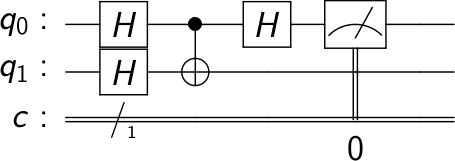
\includegraphics[width=0.5 \textwidth]{02_Background/deutsch_algorithm_circuit.png}
  \caption{Deutsch Algorithm for $f: x \mapsto x$}
  \label{figure:gate.deutsch.circuit}
\end{figure}

A quantum computer that implements this model of computing would be more powerful than any Turing machine.
It can simulate any finite physical system in polynomial time complexity, including systems with quantum effects.
The complexity class is called Bounded-error Quantum Polynomial-time (BQP).
There exists no algorithm for Turing machines to accomplish this.
%\cite{Shor1998}

